\documentclass[output=paper,colorlinks,citecolor=brown]{langscibook}

\author{Gabriella Licata \affiliation{University of California, Berkeley}}
\title{Language attitudes in Liguria: Effects of gender on the perception of Genoese}

\abstract{Impediments to intergenerational language transmission may be explained by the avoidance of a stigmatized variety by members of a social category \citep{ecke08}. Relatedly, perceptions of nonstandard or stigmatized varieties or variants may also be influenced by certain social qualities of the speakers, such as gender. Labov’s gender paradox \citeyear[261--293]{labo01} maintains that when varieties are in competition, women tend to conform to prestige forms when they are overtly prescribed but avoid those that are stigmatized. This study aims to reveal if attitudes toward Genoese are conditioned by speaker/listener gender—and how said attitudes shed light on its status and revitalization—by using the matched-guise technique \citep{lamb66}. Participants completed a survey online, rating male and female speakers of Genoese and Italian on various social qualities (locality; rurality; power; gender; solidarity; speech quality). A regression model reveals that the Italian language and male speakers overall yield higher ratings for solidarity and speech quality (p < 0.0001), though Italian-speaking females receive the highest ratings and female Genoese speakers the lowest (p < 0.0001). The matched-guise results corroborate Labov’s gender paradox, whereby women may adhere to standard (Italian) over nonstandard (Genoese) varieties when positive indexicality of the latter is limited. While women continue to be primary caregivers and language socializers of children, I argue that the results of this study pose further threats for intergenerational transmission of Genoese and current attitudes will hinder efforts to revitalize it.\\
\textit{Keywords: }language attitudes, endangered languages, sociophonetic perception, gender paradox, Genoese}
  
\IfFileExists{../localcommands.tex}{%hack to check whether this is being compiled as part of a collection or standalone
   % add all extra packages you need to load to this file

\usepackage{tabularx,multicol,multirow}
\usepackage{url}
\urlstyle{same}

\usepackage{listings}
\lstset{basicstyle=\ttfamily,tabsize=2,breaklines=true}

\usepackage{langsci-basic}
\usepackage{langsci-optional}
\usepackage{langsci-lgr}
\usepackage{langsci-gb4e}
%    \let\eachwordone=\it % Ch 14, 18

\usepackage{jambox}
\usepackage{subfigure}
\usepackage{tablefootnote}
\usepackage[nameinlink, noabbrev]{cleveref}
\crefname{enumi}{example}{examples}

\usepackage{bbding}
%\usepackage{linguex}
\usepackage{stmaryrd}

\usepackage{tipa}
\let\ipa\textipa
\usepackage{vowel}
\newcommand{\BlankCell}{}
\usepackage{ot-tableau}

\usepackage{forest}
\useforestlibrary{linguistics}
\usepackage[noeepic]{qtree}
\usepackage{pstricks, pst-xkey, pst-jtree}
\usepackage{tikz-qtree}
\usepackage{tikz-qtree-compat}
\usepackage{tree-dvips}

\usepackage{lastpage}
\usepackage{hyperref}
\usepackage{xltxtra}

\usepackage{ragged2e}
%\usepackage{subcaption}
\usepackage{floatrow}
\usepackage{float}

\usepackage[normalem]{ulem} % Pour les textes barrés
\usepackage{ifthen} 

\usepackage{todonotes}

   \newcommand*{\orcid}{}

\makeatletter
\let\theauthor\@author
\makeatother

\papernote{\scriptsize\normalfont
    \theauthor.
    \titleTemp. 
    To appear in: 
    Chad Howe and Pilar Chamorro and Timothy Gupton and Margaret Renwick.
    Theory, Data, and Practice: Selected papers from the 49th Linguistic Symposium on Romance Language
    Berlin: Language Science Press. [preliminary page numbering]
}

% Workaround for subscripts with capital letters
\newcommand{\capsub}[1]{\ensuremath{_\text{#1}}}

% Chapter 10: Table-like presentation within example environment
% classical latin > {*}late latin > old french  earlier > later   gloss
\newcommand{\montanoboxi}[7]{\parbox{2cm}{#1} > {#2}\parbox{2cm}{#3} > \parbox{1.5cm}{\textit{#4}} \parbox{1.2cm}{#5}\ > \parbox{1.2cm}{#6} \parbox{1.5cm}{#7}}
% {*}latin > earlier OF [ipa] > early OF   gloss
\newcommand{\montanoboxii}[6]{{#1}\parbox{1.9cm}{\textit{#2}} > \parbox{1.3cm}{\textit{#3}} \parbox{2cm}{#4} \parbox{2cm}{#5} \parbox{1.9cm}{#6}}

% Chapter 5
\newcommand{\redc}[1]{\textcolor{red}{#1}}
\newcommand{\bluec}[1]{\textcolor{blue}{#1}}
\newcommand{\ajout}[1]{\textcolor{blue}{#1}}
\newcommand{\ajoutplus}[1]{\textcolor{cyan}{#1}}

\newcommand{\hachure}[9]{
% Parametres :
% Coordonnees bas gauche (2 parametres) : (#1,#2)
% Coordonnees haut droit (2 parametres) : (#3,#4)
% Orientation : #5
%   1 : diagonale de pente 1
%  -1 : diagonale de pente -1
%   0 : horizontal
%   2 : vertical
% Nombre de pas horizontaux : #6
% Epaisseur du trait : #7
% Couleur : #8 (ex. green)
% Atténuation couleur : #9 (ex. 30)
\pgfmathsetmacro{\N}{#6-1}
\pgfmathsetmacro{\A}{#1}
\pgfmathsetmacro{\B}{#2}
\pgfmathsetmacro{\C}{#3}
\pgfmathsetmacro{\D}{#4}
\pgfmathsetmacro{\I}{(#3-#1)/#6}
\pgfmathsetmacro{\J}{(#4-#2)/#6}
\ifthenelse{\equal{#5}{1}}{
  \foreach \n in {0,...,\N}
    \foreach \m in {0,...,\N}
      {
        \pgfmathsetmacro{\X}{\A + ((0 + \n) * \I)}
        \pgfmathsetmacro{\Y}{\B + ((0 + \m) * \J)}
        \pgfmathsetmacro{\U}{\A + ((1 + \n) * \I)}
        \pgfmathsetmacro{\V}{\B + ((1 + \m) * \J)}
        \draw[#8!#9,#7] (\X, \Y)--(\U, \V);
      } 
  }{}
\ifthenelse{\equal{#5}{-1}}{
  \foreach \n in {0,...,\N}
    \foreach \m in {0,...,\N}
      {
        \pgfmathsetmacro{\X}{\A + ((1 + \n) * \I)}
        \pgfmathsetmacro{\Y}{\B + ((0 + \m) * \J)}
        \pgfmathsetmacro{\U}{\A + ((0 + \n) * \I)}
        \pgfmathsetmacro{\V}{\B + ((1 + \m) * \J)}
        \draw[#8!#9,#7] (\X, \Y)--(\U, \V);
      } 
  }{}
\ifthenelse{\equal{#5}{0}}{
  \foreach \n in {0,...,\N}
    \foreach \m in {0,...,\N}
      {
        \pgfmathsetmacro{\X}{\A + ((0 + \n) * \I)}
        \pgfmathsetmacro{\Y}{\B + ((0 + \m) * \J)}
        \pgfmathsetmacro{\U}{\A + ((1 + \n) * \I)}
        \pgfmathsetmacro{\V}{\B + ((0 + \m) * \J)}
        \draw[#8!#9,#7] (\X, \Y)--(\U, \V);
      } 
  }{}
\ifthenelse{\equal{#5}{2}}{
  \foreach \n in {0,...,\N}
    \foreach \m in {0,...,\N}
      {
        \pgfmathsetmacro{\X}{\A + ((0 + \n) * \I)}
        \pgfmathsetmacro{\Y}{\B + ((0 + \m) * \J)}
        \pgfmathsetmacro{\U}{\A + ((0 + \n) * \I)}
        \pgfmathsetmacro{\V}{\B + ((1 + \m) * \J)}
        \draw[#8!#9,#7] (\X, \Y)--(\U, \V);
      } 
  }{}
}

%Définition d'un pattern de type hachure
% \usetikzlibrary{patterns}
% \makeatletter
% \tikzset{hatch distance/.store in=\hatchdistance,hatch distance=5pt,hatch thickness/.store in=\hatchthickness,hatch thickness=5pt}

% \pgfdeclarepatternformonly[\hatchdistance,\hatchthickness]{north east hatch}% name
%     {\pgfqpoint{-\hatchthickness}{-\hatchthickness}}% below left
%     {\pgfqpoint{\hatchdistance+\hatchthickness}{\hatchdistance+\hatchthickness}}% above right
%     {\pgfpoint{\hatchdistance}{\hatchdistance}}%
%     {
%         \pgfsetcolor{\tikz@pattern@color}
%         \pgfsetlinewidth{\hatchthickness}
%         \pgfpathmoveto{\pgfqpoint{-\hatchthickness}{-\hatchthickness}}       
%         \pgfpathlineto{\pgfqpoint{\hatchdistance+\hatchthickness}{\hatchdistance+\hatchthickness}}
%         \pgfusepath{stroke}
%     }
% \pgfdeclarepatternformonly[\hatchdistance,\hatchthickness]{north west hatch}% name
%     {\pgfqpoint{-\hatchthickness}{-\hatchthickness}}% below left
%     {\pgfqpoint{\hatchdistance+\hatchthickness}{\hatchdistance+\hatchthickness}}% above right
%     {\pgfpoint{\hatchdistance}{\hatchdistance}}%
%     {
%         \pgfsetcolor{\tikz@pattern@color}
%         \pgfsetlinewidth{\hatchthickness}
%         \pgfpathmoveto{\pgfqpoint{\hatchdistance+\hatchthickness}{-\hatchthickness}}
%         \pgfpathlineto{\pgfqpoint{-\hatchthickness}{\hatchdistance+\hatchthickness}}
%         \pgfusepath{stroke}
%     }
% \makeatother
%~~~~~~~~~~~~~~~~~~~~~~~~~~~~~~~~~~~~~


% Chapter 7
\newcommand\pef[1]{(\ref{#1})}

\newcommand{\subscript}[1]{\textsubscript}

   %% hyphenation points for line breaks
%% Normally, automatic hyphenation in LaTeX is very good
%% If a word is mis-hyphenated, add it to this file
%%
%% add information to TeX file before \begin{document} with:
%% %% hyphenation points for line breaks
%% Normally, automatic hyphenation in LaTeX is very good
%% If a word is mis-hyphenated, add it to this file
%%
%% add information to TeX file before \begin{document} with:
%% %% hyphenation points for line breaks
%% Normally, automatic hyphenation in LaTeX is very good
%% If a word is mis-hyphenated, add it to this file
%%
%% add information to TeX file before \begin{document} with:
%% \include{localhyphenation}
\hyphenation{
anaph-o-ra
Dor-drecht
%FFI2016-76045-P-AEI/-MINEICO/-FEDE
}

\hyphenation{
anaph-o-ra
Dor-drecht
%FFI2016-76045-P-AEI/-MINEICO/-FEDE
}

\hyphenation{
anaph-o-ra
Dor-drecht
%FFI2016-76045-P-AEI/-MINEICO/-FEDE
}

    \bibliography{localbibliography}
    \togglepaper[23]
}{}

\begin{document}
\maketitle

\section{Introduction}

In bilingual communities, wherein minoritized languages are subordinated by the sustained elevation of a hegemonic language \citep{lipp97}, the study of language attitudes is vital to variation studies as it can foresee linguistic behavior (\cite{coop77}; \cite{garr03}). For example, impediments to intergenerational language transmission may be explained by members of a social category avoiding a perceived stigmatized or nonstandard variant or variety and thus indexical field of social meaning \citep{ecke08}, as listeners are strikingly perceptive when it comes to identifying social aspects of speakers (e.g. gender or education level) via their speech \citep{chap16}. Nevertheless, if people are plainly and directly asked what they think about a particular language variety or variant, the chances are higher that their answers highlight conscious shared and communal stereotypes rather than discrete, individual ones \citep{stef05}, thus gauging language attitude trends from ethnographic and experimental perspectives alike is crucial for understanding the ideologies that inform or hinder efforts of language restoration and revitalization. Whereas early methods ranged from direct questioning in surveys and interviews, the value placed on the importance of language attitude tests has evolved to uncover subconscious judgements of a variety or variant \citep{garr01}. Results shed light on the overt and covert language ideologies that prioritize a language in a given context. The matched guise test (see \cite{lamb66}) is considered to be an indirect approach because participants are not aware that they may hear the same speaker producing the targeted varieties or variants \cite{soli02}. They are also unaware that the attributes they apply to each speaker will be later interpreted into ideologies towards the variety or variant \citep{garr01}.
\par The historical and present-day institutional consideration of language varieties bears great weight on the manners in which speakers use and perceive them, which in turn reiterate collective and individual attitudes. The several regional languages that continue to be spoken (to varying degrees) in Italy are referred to as dialects, a demeaning and problematic misnomer \citep{fish91}, particularly because said “dialects” receive little to no institutional support and several are at risk of extinction \citep{colu09}. The endangerment of these varieties is a “social hurt” to Italian communities \citep{fish91}, indicative of social injustice via restrictive monolingual language policies. However, some social stigma towards these regional languages has lessened, causing risorgenze dialettali \citep{berr06}, or dialectal resurgence. Hence, understanding the social variables that condition attitudes towards these varieties are of paramount importance when considering their potential revitalization.

\begin{figure}
    
\includegraphics{figures/licata_fig1.eps}
    \caption{Italy divided by regions, Liguria highlighted\protect\footnotemark}
    \label{fig:licata:01}
\end{figure}

\footnotetext{Map by TUBS licensed under CC BY-SA 3.0 (\url{https://en.wikipedia.org/wiki/File:Liguria_in_Italy.svg})}
\par The present research seeks to quantitatively assess covert language attitudes towards Genoese (o zeneize/zeneise), an endangered dialect of the Gallo-Italic language Ligurian in Northwest Italy with approximately 400,000 speakers in the region of Liguria (see \figref{fig:licata:01}). This study aims to empirically uncover language attitudes towards Genoese and standard Italian in Liguria by using a matched guise test, seeking to understand if attitudes toward Genoese and Italian are similarly conditioned by speaker gender and/or listener gender. Given Genoese’s endangerment and the lack of institutional support at local, regional, and national levels, modern attitudes towards Genoese that may act as either barriers or gateways for its revitalization will be discussed in light of the results.



\section{Literature review}
\subsection{Sociophonetic perception and gender}
Language ideologies associate the social constructs to those of language; that is, there exists a naturalized nexus between a speaker (or group of speakers) and a linguistic variety or variant \citep{gals95} that indexes social meaning. Take for instance the phenomenon of /t/ release in American English, which has been associated with nerdy high school girls \citep{buch01}, gay men in San Francisco \citep{pode06}, and Orthodox Jewish boys \citep{buni01}. While this variant can index stagnant qualities, like intelligence, education, or exasperation, the true meaning of the variant is dynamic and depends on its speech group and context in place and time. However, an index’s stagnant qualities call attention to the indirect indexicalities \citep{ochs90} that reveal fossilized ideologies that purport naturalized language behavior by a particular identity group \citep{ecke99}.  Earlier work in feminist linguistics examined how speaker sex was the linguistic divide that separated women from men, and whether or not these speech differences were examined in light of societal or economic inequities, these early descriptions of language use failed to address the construct of gender as shaping language use. Later research reveals how binary interpretations of sex conflated binary interpretations of gender that essentialized how males/men/boys and females/women/girls should behave and speak. \cite{butl02} challenged binary categories of both sex and gender, ultimately revealing how the latter can constitute a fluid identity that is performed and reiterated in language choice in varying contexts, among other communicative and social mechanisms.
\par A Peircean approach to analyzing the semiotics of a culture and community provides information on how social constructs like gender are created and maintained in discursive context \citep{ochs90} and how ideologies derive from indexes and serve as “metadiscourses that comment on and regiment other communicative practices” \citep{gals02}. Thus, constructs like gender must be examined within their context, for example, Western capitalist cultures have traditionally viewed sex and gender as synonymous features of humans. Sex is socially constructed as gender, and an overview of gender semiotics in Italian culture and the restrictions of expression in Romance languages reveal the conflation of the two, thus the identities of woman and man are interchangeable with the genders female and male (respectively). In societies that favor and maintain a binary gender system (e.g. Italy) in language and culture alike, both production and perception studies have attested patterns of linguistic behavior mediated by speaker identification with male or female genders. In such a society with gender-specific roles for men and women, the indexes of those genders become entrenched in the semiotics and ideologies of the female and male sexes. Thus, the linguistic patterns of female- and male-gendered speakers – among other social characteristics – of a variety can apprise linguists on who has access to positive indexical fields related to a language or variant. Labov’s theory of gender paradox \citep{labo01} states that women conform to prestige uses of language when said forms are overtly prescribed and avoid those that are stigmatized. However, men may access nonstandard variants or varieties as a feature of solidarity, enjoying the assigned covert prestige as a member of a particular social group \citep{trud72}, in which [working-class] men esteem their own nonstandard ways of speaking as a necessity of social status, while women lean towards toward use of the standard. One interpretation for the linguistic behavior of the latter social group is that women use language as symbolic capital \citep{schi98} within a capitalist economic system wherein clearly-designated gender roles enforce a power imbalance that favors men \citep{fede04} – a plausible explanation as to why “women show a lower rate of stigmatized variants and a higher rate of prestige variants than men” \citep{labo01}, as prescriptive, standard language use may index education and socioeconomic status.

\par Recently, empirical studies have demonstrated trends in in the sociophonetic perception of male- and female-identifying speakers favoring certain language varieties or variants. Since to our knowledge there are no such studies assessing language attitudes towards regional varieties in Italy, parallel studies concerning minority languages and nonstandard variants in other countries and languages with similar semiotic structures to Italy can provide attestations that lend support to the maxims of the gender paradox theory. \cite{lour13} used a matched guise test to examine adolescent attitudes towards standard and vernacular Galician in rural and urban communities. They found that standard Galician (henceforth SG) is rated more prestigious than vernacular Galician (VG) by urban student listeners, even though they have less access to the language compared to rural student listeners. Also, SG is rated more positively when spoken by male speakers as it’s considered an elite marker of local male politicians, though Galician overall received low positive ratings by female listeners. In \cite{chap16} study of nonstandard intervocalic /s/ voicing in Costa Rican Spanish, stimuli of both male and female speakers were manipulated in order to contain both voiceless and voiced tokens ([s] and [z], respectively). Female speakers were evaluated as less educated and of a lower class when their speech contained the nonstandard form [z]. Thus, with no positive gains to be had, women can avoid variants that do not provide them with opportunities for positive indexicality. Indexical systems (see \cite{silv03};\cite{ecke08}) lay the groundwork for the communicative semiotics of a culture, whereby different genders hold different roles in society. In most Western cultures, women spanning multiple generations are still the primary social reproducers, and thus they are the principal language socializers of children – especially in the early years of acquisition – and provide the largest amount of verbal input to children \citep{pere03}. Thus, if women attribute unattractiveness to a particular variety \cite{cava06} and render it less powerful in regards to social capital, they can become instrumental in leading linguistic shift towards a more standardized, prestige variety.

\subsection{Italian and Italy’s “dialects”}
\par Investigating language attitudes in bilingual environments is of particular importance in cases where the language vitality of one language is steadily or rapidly decreasing. Italy’s regions were linguistically divided for centuries – each had its own distinct language and corresponding dialects – even after unification of the Italian state in 1861, when standard Italian was found in the form of fiorentino (Florentine). \cite{akma17} discuss the coining of regional languages in Italy as “dialects” precisely during the unification and enforced during the fascist era as a means to denigrate their social value and utility. The most recent census of “dialect”-only speakers counts them at 14.1\% (a decrease of more than half since 1988), and bilingual Italian and “dialect” speakers forming 32.2\% of the general population, \citep{ista15}, with further reports tying the use of “dialects” within the family and to a low-level education (i.e., middle school). UNESCO’s document titled Language Vitality and Endangerment \citep{bren03} offers various measures of language vitality under the section Nine Major Evaluators of Language Vitality\footnote{UNESCO’s assessments generally rate from 0--5, with 0 signifying language extinction and 5 signifying safe and universally spoken (i.e., language is safe from turning obsolete). For an in-depth understanding of the parameters and document in general, visit \href{http://www.unesco.org/new/en/culture/themes/endangered-languages/language-vitality/}{http://www.unesco.org/new/en/culture/themes/endangered-languages/language-vitality/}}. \citep{colu09} applied these parameters to several of Italy’s regional languages and calculated an average score of 2.6 (out of 5), which deems the varieties somewhere between critically endangered and severely endangered.
\par With regards to the maintenance of minority or less prestigious languages such as regional languages in Italy, it is important to understand how collective behaviors and attitudes towards a language variety or variant are carried out in order to address how macro-level trends operate at the micro-level, such as within the community, family, or individual. In \cite{cava06} ethnographic study of language shift in the Lombard city of Bergamo, she found that the local vernacular, Bergamasco, is notably implicated in sociolinguistic negotiations of whether or not to maintain the language’s vitality, and significant to this is the role of gender reiteration in linguistic practice. Bergamasco is often linked to working-class male identity while Italian is linked to female identity of any given class. In this study, \citeauthor{cava06} found that during the 1950s and 1960s, female social reproducers – a.k.a. the mothers and grandmothers – as the primary caregivers were expected to teach Italian to their children, even if Bergamasco was their native and dominant tongue, a practice inherently opportunistic in socioeconomic advancement (p. 200). The possibility of code-switching or bivalent varieties \citep{wool98} was and still is not an option, as a purest attitude of language is prevalent in both language groups. \cite{cava06} concludes that the gendered indexicalities of Bergamasco language use is one example of why it is not being passed down to the younger generation and therefore dying out, but is dissimilarly vibrantly maintained among the city’s adult male population, particularly those of the working class, with a frequency of use of nearly 95\%. Gendered linguistic stigmatization, coupled with a lack of intergenerational transmission, are accordingly two major factors in the loss of regional varieties throughout Italy.

\subsection{On the status of Genoese}
\par The institutional planning that underpins language standardization and a monolingual society seeps into the attitudinal treatment of other coexisting languages (i.e. those of minority or of nonstandard status and, in the case of several regional languages in Italy, those which are vulnerable to extinction). Genoese, dialect of Ligurian, distributed both in coastal, urban and rural areas (see red area in \figref{fig:licata:02}) is under the stewardship of the older generations and not 

\begin{figure}
    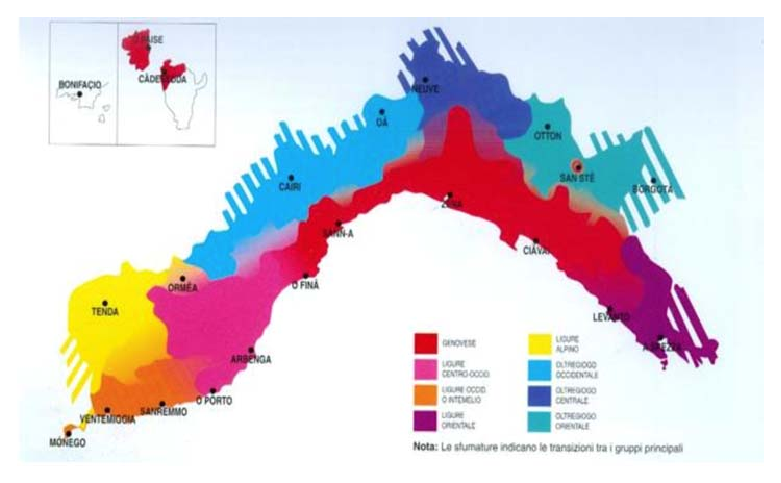
\includegraphics[scale=0.9]{figures/licata_fig2.eps}
    \caption{Dialectal map of Ligurian varieties \citep{toso99}}
    \label{fig:licata:02}
\end{figure}

being transmitted to younger generations. To date, no structures are in place to gauge an approximate number of Genoese speakers – nor other Italian “dialects” – on the ISTAT, Italy’s main producer of statistics. Measures to collect these data are costly and rare, though local language activists estimate that 25\% of the Ligurian population speaks Genoese and the large majority of these speakers are believed to be older \citep{acqu18b}. If the language continues to lose one fourth of speakers for each generation (as it has been, more or less), then at the end of this century, no more than 15\% of the population will be able to speak Genoese, and likely a more Italianized form \citep{colu09}. \cite{colu09} assessment of Genoese by UNESCO standards (see \cite{bren03}) is not dramatically different than the average score of all regional languages (~2.1). While there is a significant amount of research on Genoese (\cite{toso99}; \cite{gism55}; \cite{forn88}; \cite{cost93}, among others), these texts are mainly written from a linguistic perspective. The resources available for people learning Genoese for non-research purposes are scarce, and vary from one to another, that is, there is no “standard” for accessible materials \citep{acqu18a}. Furthermore, there do not seem to be any grammar materials available for children\footnote{The teaching of Genoese to children is uncommon, but what is in motion is domain-specific, i.e., theatre productions in Genoese.}.  Without diffusion to younger generations in school and home, Genoese is slowly on its way to extinction, as little is being done to revitalize the variety at a legislative level that would ensure some practice of intergenerational transmission, even if outside of the home.

\section{Methodology}
The current sociolinguistic status of Genoese is unclear, though qualitative evidence collected by language activists and community members has shed light on the need to take dramatic steps to revitalize the variety. The current study, with its employment of a matched guise experiment, uncovers some of the covert attitudes towards Genoese and Italian in the Ligurian region, providing vital information on who has access to positive indexical fields in the employment either variety.

\subsection{Guises and stimuli}
The two guises in this experiment are native Italian/Genoese speakers, one self-identified female and the other a self-identified male, both in their mid-thirties and married to one another. Both were born and raised in or around Chiavari, a coastal city approximately half an hour south of the city of Genoa, and both continue to reside in Liguria. Both are medical professionals and speak Italian and Genoese on a daily basis, both in the home and at work (the latter language, with older patients when it facilitates conversation). Using a Zoom H2 Handy Recorder, the guises were recorded reading an excerpt from The Little Prince, translated into Italian and Genoese and entitled Il piccolo principe and O Prinçipe picin, respectively \citep{desa15}. The two guises read the excerpt in Italian and Genoese, for a total of four audio samples.

\begin{figure}
    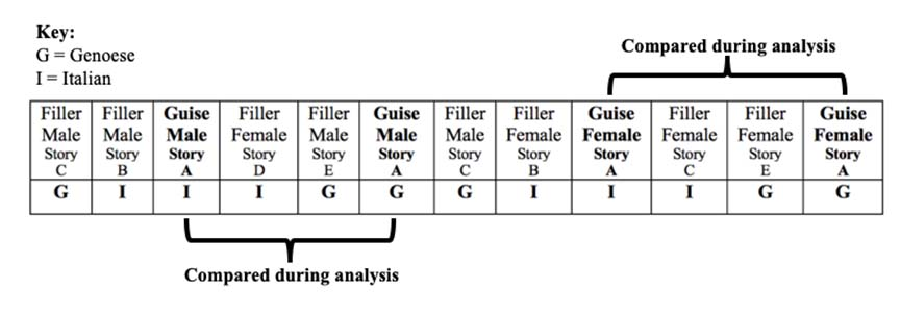
\includegraphics[scale=0.8]{figures/licata_fig3.eps}
    \caption{Single group of judges for matched guise experiment, two guises, two varieties \citep{stef05}}
    \label{fig:licata:03}
\end{figure}

As an attempt to minimize suspicion of similarity of both the male- and female-gendered guises in Italian and Genoese in the recordings, they were separated by eight other audio samples from eight unique speakers composed of four female- and male-identifying speakers, with each gender group having two native Italian speakers and two native Genoese speakers, reading other excerpts from the book, each in Italian and Genoese. Participants were told that they would be listening to twelve different speakers, when in reality there were only ten. The audio samples were organized for a single group of judges \citep{stef05}, meaning that all participants hear and rate all audio samples (see \figref{fig:licata:03} above).

\par Sixty-five participants (33 female-identifying, 32 male-identifying) completed the experiment online. Demographic information is presented in \tabref{tab:licata:01} below. All participants were between the ages of 20–40 and grew up in Liguria and at the time of the study and still lived there. In addition to 

\begin{table}
\begin{tabularx}{\textwidth}{XX}
\lsptoprule
\textbf{Participant information}\\ \midrule
Mean/median age (in years) & 29/29 \\
Ratio female : male (n) & 33:32 \\
Mother tongue(s) (n) & Italian (65); Italian with: English (7); French (6), Genoese (4); Spanish (1); Biijinolu\footnotemark (1) \\
Frequency of Genoese spoken in household during youth (n) & Yes, often (29); Every so often (16); Not often (11); Never (9) \\  
\lspbottomrule
\end{tabularx}
\caption{Participants’ demographic and linguistic information}
\label{tab:licata:01}
\end{table}

\footnotetext{Biijinolu is a dialect of Ligurian spoken in the town of Buggio, Commune of Pigna, Province of Imperia, bordering France.}
location, this group was preferred for two reasons: 1) they are either having children or will be the next generation to do so; and 2) they are speaking more Italian than Genoese. As language socializers of the youngest or next generation of Ligurians, it will be this Italian-speaking age group that will be instrumental in a revitalization of Genoese, if they are invested in doing so.

\subsection{Experiment design}
\label{sec:3.2}
Participants were asked to complete the experiment using Qualtrics \citep{qual13}, an online survey platform, in a quiet room with headphones to reduce the variability of distraction and influence from those who might be around. Participants were also asked to complete the experiment in one sitting, and this was achieved by using features in Qualtrics that did not allow participants to backtrack to previous pages nor save their work and return to it at a later time. Participants generally took between 40–50 minutes to complete the experiment.
\par The experiment was uploaded into Qualtrics and sent to participants via email. Though collecting the data in-person would allow me to control for quality (i.e., assure a quiet room; all participants wearing headphones; assistance with any questions), the facilitation of this particular software allowed me to collect a large amount of data in an organized and consistent fashion. All participants completed two screening questions prior to starting the experiment in Qualtrics. These questions assured that participants were raised and continue to reside in Liguria and were between the ages of 20–40. To understand the background behind the participants’ ratings, simple demographic questions (age; gender) were asked as well as a light linguistic background and frequency of Genoese spoken in household growing up. Participants then proceeded to the matched guise test, and were told that they would hear twelve distinct voices reading passages from a story. Participants were also prompted to assess the speaker based on a series of social qualities. Using a 7-point Likert scale (see \figref{fig:licata:04}), speakers were evaluated based on the following characteristics:
\begin{itemize}
    \item [P1.] \textit{antipatica/simpatico} (rude/nice)
    \item [P2.] \textit{istruita/non istruita} (educated/not educated);
    \item [P3.] \textit{parla bene la lingua/non parla bene la lingua} (speaks language well/does not speak language well);
    \item [P4.] \textit{dubbioso/affidabile} (untrustworthy/trustworthy)
    \item [P5.] 	\textit{era nato/a in Liguria/fuori da Liguria} (was born in Liguria/outside of Liguria)
    \item [P6.]	\textit{non sarebbe il mio amico facilmente/sarebbe il mio amico facilmente} (would not easily be my friend/would easily be my friend)
    \item [P7.]	\textit{dalla città/ campagna} (born in the city/born in the country)
    \item [P8.]	\textit{ha una voce maschile/femminile} (has a masculine/feminine voice)
    \item [P9.] 	\textit{spiacevole di ascoltare/piacevole di ascoltare} (not pleasant to listen to/pleasant to listen to)
    \item [P10.]	\textit{ha un accento fino/brutto} (has a refined accent/has an ugly accent)
    \item [P11.]	\textit{ha un lavoro che paga molto/poco} (has a high-paying/low-paying job)
\end{itemize}

A rating of “1” and “7” indicate a choice of either polar extreme, while 2/3 and 5/6 demonstrate the gradient nature of such a scale. An option of no opinion was offered in the middle of the 
scale (“4”).

\begin{figure}
    
\includegraphics[scale=0.75]{figures/licata_fig4.eps}
    \caption{Likert scale prompt in Qualtrics$^{\text{\textregistered}}$}
    \label{fig:licata:04}
\end{figure}


\subsection{Statistical analysis}
I converted raw data from the Likert ratings into z-scores in order to normalize the scale. The ratings of aforementioned question prompts were then grouped into six dependent 
variables, demonstrating attributes of: 1) locality (P5); 2) rurality (P7); 3) power (P2; P11); 4) solidarity (P1; P4; P6); 5) gender (P8); and 6) speech quality (P3; P9; P10). The ratings from the male guise (henceforth, MG) speaking Italian and Genoese were compared to one another in \citep{rcor18} using the lmerTest package \citep{kuzn17} mixed effects linear regression model, and also those of the female guise (FG). One regression model was run for each dependent variable and I tested for the effects of three social factors: self-identifying gender of speaker (male/female), self-identifying gender of listener (male/female), and language variety (Genoese/Italian). Individual participant was included as a random effect.


\section{Results}
A total of 65 surveys were obtained and each participant rated the 12 voices with the same series of questions (see \sectref{sec:3.2}). Of the six regression models, three showed a significant effect of either gender or language alone, or an interaction thereof. Results are reported in the tables below, with the intercept being Female/Genoese-speaking. Significant differences in ratings are further detailed in the following graphics and dependent variables with significant findings will be discussed separately.

\subsection{Gender attribute}
\par The gender attribute quality tests for differences in the perceived social traits of masculinity and femininity. While there was no interaction of guise language and either speaker or listener gender (see \tabref{tab:licata:02}), participants overall rated female speakers as sounding more feminine, and male speakers as sounding more masculine (p < .0001), indicating that the former do not sound more masculine when speaking Genoese (see \figref{fig:licata:05}). This interpretation of perceived “genderness” will be discussed later on in regards to access to Genoese indexical fields.

\begin{table}
\begin{tabularx}{\textwidth}{lrrrr}\lsptoprule
                     & $\beta$ & \textit{SE} & \textit{T} & \textit{P} \\ \midrule
(Intercept)\footnotemark          & 0.974   & 0.040        & 23.948     & <.0001     \\
GL Italian\footnotemark         & 0.017   & 0.054       & 0.305      & 0.761      \\
GG Male              & –1.920   & 0.045       & –43.113    & <.0001     \\
LG Male              & –0.069  & 0.049       & –1.416     & 0.159      \\
GL Italian : GG Male & –0.009  & 0.063       & –0.140     & 0.888      \\
GL Italian : LG Male & 0.042   & 0.063       & 0.659      & 0.511   \\  
\lspbottomrule
\end{tabularx}
\caption{Summary of mixed effects linear regression model fitted to gender attribute ratings}
\label{tab:licata:02}
\end{table}

\footnotetext{The intercept is female listeners rating female guises speaking Genoese. Positive $\beta$ indicate more feminine ratings.} 
\footnotetext{Abbreviations as follows: GL = guise language; GG = guise gender; LG = listener gender}

\begin{figure}
    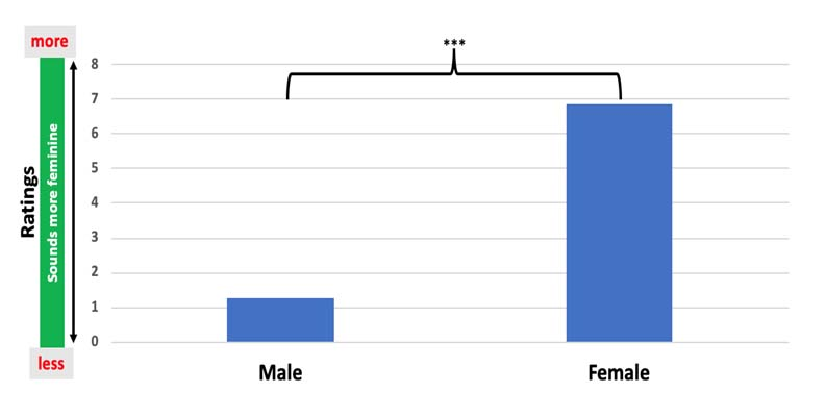
\includegraphics[scale=0.9]{figures/licata_fig5.eps}
    \caption{Gender attribute ratings assigned to guise language}
    \label{fig:licata:05}
\end{figure}



\subsection{Solidarity}
The social attribute of solidarity specifies how closely tied the listener may feel towards the speaker, i.e., how likely they are to have the speaker in their various social circles. Results of this regression model reveal that listeners rated Italian speakers higher for solidarity (p < 0.001) than Genoese speakers (see \tabref{tab:licata:03} and \figref{fig:licata:06}). Furthermore, with respect to listener-gender, male listeners overall give higher ratings for solidarity (p < .02) as demonstrated in \figref{fig:licata:07}. Approaching significance were higher ratings for male speakers overall (p < .052), however, also approaching significance were slightly lower ratings for Italian-speaking males (p < .052).

\begin{table}
\begin{tabular}{lrrrr}\lsptoprule
                     & Β      & \textit{SE} & \textit{t} & \textit{P} \\ \midrule
(Intercept)          & –0.485 & 0.157       & –3.091     & <.002      \\
GL Italian           & 0.546  & 0.167       & 3.274      & <.001      \\
GG Male              & 0.268  & 0.137       & 1.957      & 0.052      \\
LG Male              & 0.452  & 0.201       & 2.247      & <0.027     \\
GL Italian : GG Male & –0.378 & 0.194       & –1.954     & 0.052      \\
GL Italian : LG Male & –0.205 & 0.194       & –1.059     & 0.291      \\
\lspbottomrule
\end{tabular}
\caption{Summary of mixed effects linear regression model fitted to solidarity ratings}
\label{tab:licata:03}
\end{table}

\begin{figure}
    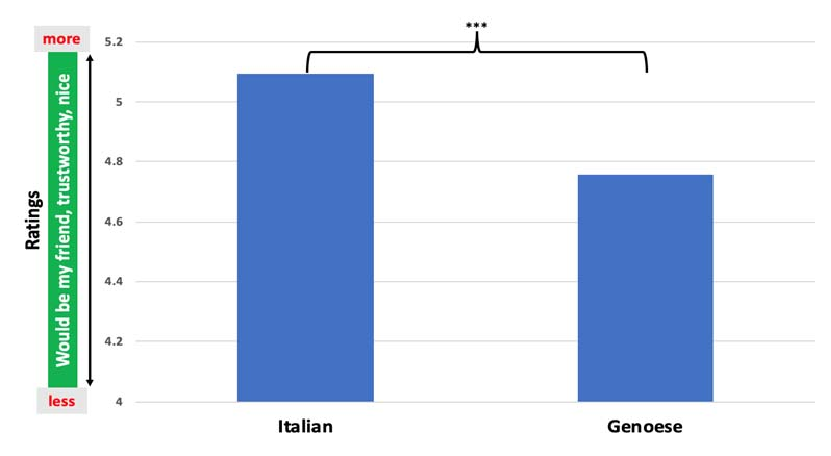
\includegraphics[scale=0.8]{figures/licata_fig6.eps}
    \caption{Solidarity ratings assigned to guise language}
    \label{fig:licata:06}
\end{figure}

\begin{figure}
    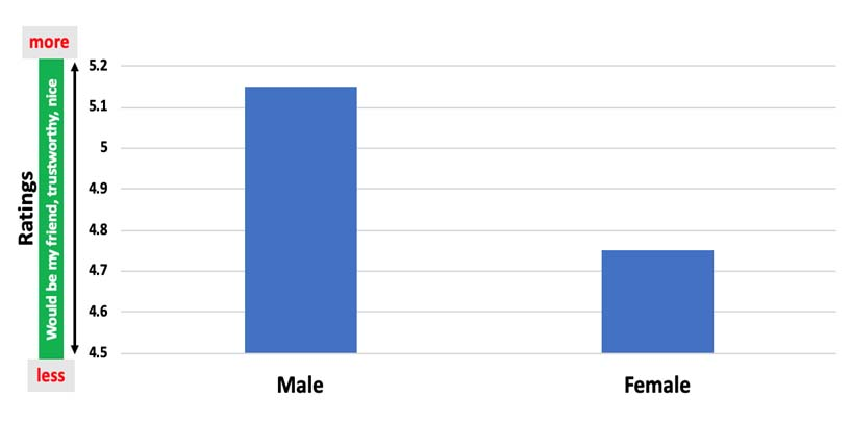
\includegraphics[scale=0.8]{figures/licata_fig7.eps}
    \caption{Solidarity ratings by listener gender}
    \label{fig:licata:07}
\end{figure}

\subsection{Speech quality}
Recall that the category of speech quality required listeners to assign ratings based on command of language, pleasantness of voice, and accent. Both main effects and interactions of language and speaker/listener gender arose as significant (see \tabref{tab:licata:04}). All listeners afforded higher ratings to Italian speakers over Genoese speakers (p < 0.001), and furthermore, listeners rated Genoese-speaking females lower than Italian-speaking females and Genoese-speaking males (both p < .001), though Italian-speaking females were rated higher in this category than Italian-speaking males (p < .001). These results (see \figref{fig:licata:08}) suggest that Genoese-speaking females are penalized in the speech attribute category.

\begin{table}
\begin{tabular}{lrrrr}
\lsptoprule
                     & Β      & \textit{SE} & \textit{t} & \textit{P} \\
\midrule
(Intercept)          & –0.491 & 0.148       & –3.321     & <.0010     \\
GL Italian           & 1.032  & 0.176       & 5.860      & <.0001     \\
GG Male              & 0.529  & 0.144       & 3.660      & <.0003     \\
LG Male              & 0.002  & 0.183       & 0.013      & 0.9890     \\
GL Italian : GG Male & –1.133 & 0.204       & –5.543     & <.0001     \\
GL Italian : LG Male & –0.031 & 0.204       & –0.153     & 0.8790     \\
\lspbottomrule
\end{tabular}
\caption{Summary of mixed effects linear regression model fitted to speech quality ratings}
\label{tab:licata:04}
\end{table}



\begin{figure}
    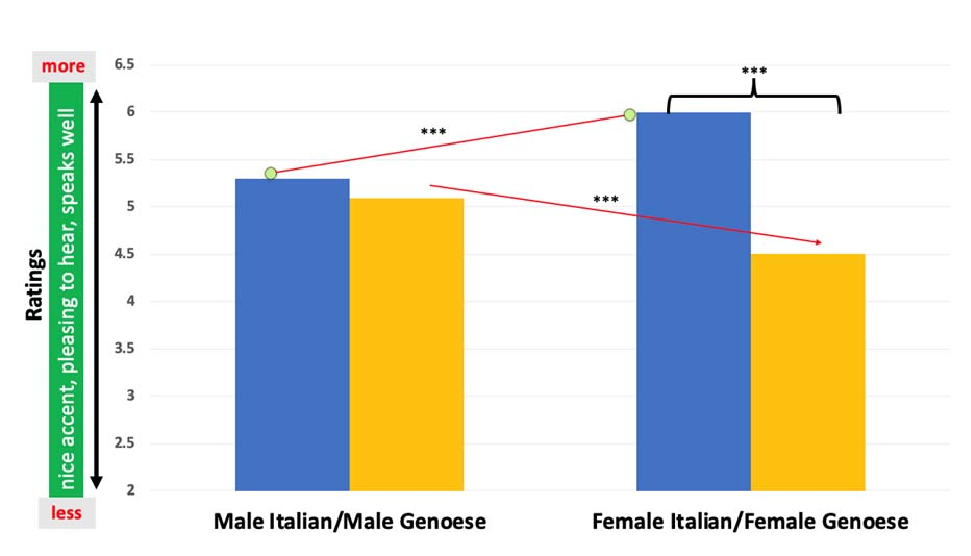
\includegraphics[scale=0.7]{figures/licata_fig8.eps}
    \caption{Speech quality ratings assigned to guise language conditioned by speaker gender}
    \label{fig:licata:08}
\end{figure}

\section{Discussion}
The experiment elicited covert attitudes towards the Genoese and Italian speech of male and female guises by employing the matched guise design, an indirect methodology that aims to uncover said attitudes without any explicit questioning. After assessing the ratings of six major social qualities – locality; rurality; power; solidarity; gender; and speech quality – significant results of Ligurians’ ratings towards both Italian and Genoese reveal attitudes that may lie below the level of consciousness. In light of these variables, the data can inform us of how these listener-participants and Ligurians in general perceive both male and female speakers of Genoese and Italian in this region of Italy. Gender judgements overall aligned with the expressed gender of the guises – the male guise was judged as more “masculine-sounding,” and the female as more “feminine-sounding.” In Italian culture, wherein femininity in speech is attributed to women, and masculinity to men, these results may be considered a positive result in light of who has positive entry into the indexical field of Genoese in the Ligurian region; men are often the face of those speaking and writing in Genoese, and all the major players working on revitalization are men. If the variety is associated with a male identity, yet female identities are not evaluated as sounding more masculine when speaking it, then there is no barrier to entry for those female speakers who wish to index a more “feminine” indexical field in Genoese.
\par The ratings towards Italian in the category of solidarity were significantly higher than those of Genoese, which affiliate well with trends in language use. Most of my listeners did not actively nor regularly speak Genoese, and even though several might be considered heritage speakers of Genoese, the language is linked to older generations and private spaces, like the home of a grandparent, and Italian is reserved for private and public spaces, including the immediate home, workplace, and school. Solidarity functioning as a social indicator may demonstrate gender disparity, favoring men over women in terms of covert prestige to a variety (\cite{labo72}; \cite{trud72}). Stemming off of the notion that solidarity to a group is often linked to men, who perhaps have less need to use language as social capital, male listeners yielded higher solidarity ratings overall (to both languages) and results approaching significance in this category also reveal that higher ratings were allotted to male speakers overall. Interestingly, lower ratings towards Italian-speaking males were approaching significance, hence more data may reveal more interactions, as it is possible that although Italian received significantly higher solidarity ratings, male speakers of Genoese may be a subgroup that also receives higher assessments, a result that would support the theories proposed by \cite{labo72} and \cite{trud72}. 
\par The results in the speech quality category shed light on the stratification of both language and gender of speaker/listener. While all Genoese speakers were given lower ratings than their Italian counterparts, female Genoese speakers’ low ratings were most severe, followed by male Genoese speakers, then both female and male Italian speakers, respectively. In Italian culture, whereby gender and sex as constructs are intrinsically linked, these results are similar to \citeauthor{cava06}’s ethnographic findings \citeyear{cava06} of gendered prescriptive language use in Bergamasco, as female speakers prefer to use a standard language variety that allows for positive indexicality and eschew a stigmatized language variety if causes the indexical field to be obstructed, which in turn would also weaken any solidarity among Genoese-speaking females as a community of speakers. These findings are argued to corroborate Labov’s gender paradox \citep{labo01}, whereby female speakers adhere to (and are identified with) the standard variety (Italian) over the nonstandard (Genoese) when positive indexicality of the latter is limited, as opposed to male speakers who may index both with less detriment.
\par While the independent variables of gender and language did not bear any significant results on locality, rurality, and power, the first may be explained by the fact that Genoese speakers did not sound more local-sounding than Italian speakers; that is, it is possible that the Italians also had a local-sounding accent that pertains to Liguria. Furthermore, based on the geography of Liguria (see \figref{fig:licata:01}), while Genoese has been linked to more rural communities with older populations, the region is long and slender, thus movement from the coast towards the mountains is easy and frequent for many commuters to the more bustling coastal areas. Genoese is also maintained vibrantly, and with some prestige, in urban and coastal areas where older populations have been established, particularly in the city of Genoa. The fact that neither language nor gender produced any significant effects on the power ratings is a positive result when considering prestige; Genoese does not point to an index of lower education nor less income. This is in contrast with qualitative accounts of Genoese and Italian “dialects” in general, which are often deemed ‘low’ varieties \citep{colu09} and symptomatic of backwards movement in an ever-globalizing world where the English language symbolizes social capital. Thus, the lack of significance with this variable is a positive outcome, and may support a refocusing of the regional agenda\footnote{It is worth noting that the revival of regional languages in Italy has been linked to rising populist movements, particularly in the North, where the Lega Nord political party (center-right) has used language revitalization as a tactic in a larger strategy to reprioritize local over national and global. See \cite{ruzz08} for an in-depth discussion on ethno-national goals of language maintenance and identity in Northern Italy.}  on localized efforts to revitalize Genoese.
\par The quantitative results present an ideological paradox of covert attitudes towards Genoese, an endangered variety with no official status in Liguria. \citeauthor{cava06}’s ethnographic account \citeyear{cava06} found similar trends in the Bergamasco / Italian confront. Women in Bergamo, through their role as caregivers and the linguistic responsibility associated with this role, have become increasingly associated with Italian language indexes, while Bergamasco has become a language of solidarity among men, with regards to practice and perception. There is also a clear division of sociolinguistic labor; men are generally not responsible for how children speak in early socialization – their linguistic responsibility is saving Bergamasco, and they dominate linguistic revitalization activities \citep{cava06}. The variable speech quality proves critical for assessing the future vitality of Genoese, as women are still the primary caretakers of children and thus most influential in language socialization, hence the impact in early years of language acquisition \citep{poto08}. Furthermore, with women – who continue to inhabit the role of primary social reproducer in Italy – effectively absent from revitalization efforts of Genoese in Liguria, I argue that the results of the present study pose immediate threats to the future language vitality of Genoese.

\section{Conclusion}
The present study has sought to obtain covert attitudes towards the Genoese and Italian language varieties of the Liguria region in Italy using an indirect method in the form of a matched guise test. Several of Italy’s regional languages are stigmatized, do not have a consensus on a unified, more standard form, and have little to no institutional safeguards. The results of this study support the theory of gender paradox in that women avoid the stigmatized, nonstandard variety. When judged on their quality of speech and language use, Genoese-speaking women are rated lower than Italian-speaking women and men overall. As they cannot positively access the indexical field Genoese with respect to these social attributes, they will utilize the standard language – Italian – and will pass it down as the dominant language to the next generation as the primary caregivers in the home and wider society. In spite of this disparity, a small renaissance of revitalization is occurring all over Liguria, however, in small and fragmented efforts. Nevertheless, this study would benefit from being expanded to assess both covert and overt attitudes of more participants in order to have a broader picture of generalized attitudes towards the use and maintenance of Genoese and its potential support as well as implications for revitalization. Genoese varies in its form (mostly lexical) from province to province, thus including guises that speak different forms of Genoese is necessary measures to take when evaluating collective attitudes in the future.

\section*{Acknowledgments}
I would like to express my gratitude to family and friends in Liguria who assisted in this project, especially Monica Rossi and Davide Proletti and family (Daniel, Benedetta, Daisy), Daniele Picetti and Valentina Monteverdi, and Giovanni Picetti, Elena Delucchi. Thank you to all those who either provided audio or participated in the survey. Lastly, thank you to Dr. Justin Davidson (UC Berkeley) for his immense help in experiment design, statistical analysis, and editing.

\nocite{*}
\printbibliography[heading=subbibliography,notkeyword=this]

\end{document}
